%!TEX root = ../thesis.tex
%*******************************************************************************
%****************************** Sixth Chapter *********************************
%*******************************************************************************

\chapter{Discussion}  %Title of the Sixth Chapter
\label{chp:discussion}
\clearpage

\newpage\null\thispagestyle{empty}\newpage


% \par \acrfull{t2d} is a chronic metabolic disorder characterized by peripheral insulin resistance and a relative insulin deficiency. A critical facet of \gls{t2d} is the progressive dysfunction of pancreatic islet $\beta$-cells that secrete insulin which plays an indispensable role in the regulation of glucose homeostasis. The onset of $\beta$-cell dysfunction in \gls{t2d} may involve different but synergistic mechanisms which may trigger inflammation. The chronic, low-grade inflammation of metabolic tissues, including pancreas and pancreatic islets, is now considered to be a part of the etiology of \gls{t2d}. Cross-talk between immune cells and $\beta$-cells in turn can initiate a vicious cycle of $\beta$-cell dysfunction. However, our understanding of the dynamics of islet immune cell infiltration during \gls{t2d} progression is incomplete as no focused analysis of immune cell signatures has been performed and time-course data in informative animal models are missing. While the role of islet-resident macrophages in maintaining islet homeostasis and driving islet inflammation has been appreciated for quite a while, knowledge about their phenotypes and their dual role \\

\par \acrfull{t2d} is a complex disorder accounting for over 90\% of all diabetic cases worldwide \textbf{\cite{home_idf_nodate}}. In \gls{t2d}, increased blood glucose levels, or hyperglycemia, is the result of the body's inability to respond fully to insulin, a condition termed insulin resistance. The onset of insulin resistance increases the demand on $\beta$-cells, leading to heightened synthesis and secretion of the hormone. In some individuals, chronic insulin demand eventually results in $\beta$-cell dysfunction and failure, leading to overt \gls{t2d} \textbf{\cite{banday_pathophysiology_2020}}.\\

\par Obesity and aging are key risk factors for \gls{t2d}, and both conditions are associated with persistent, low-level inflammation in metabolic tissues, including pancreas and pancreatic islets \textbf{\cite{schulze_dietary_2005,donath_inflammation_2013,lee_integrated_2018,ying_role_2019}}. This type of inflammation is often referred to as metaflammation in obesity and inflammaging in aging, and are now considered to be a part of the etiology of \gls{t2d} \textbf{\cite{prattichizzo_inflammageing_2018}}. Crosstalk between immune cells and $\beta$-cells under metabolic stress can initiate vicious cycles of $\beta$-cell damage \textbf{\cite{cosentino_crosstalk_2021}}. While accumulating evidence has implicated the innate immune system, particularly islet-resident macrophages, in driving the metabolic-stress induced inflammation, discrepancies about their nature, number and inflammatory markers in islets of \gls{t2d} patients and rodent models still exist \textbf{\cite{eguchi_islet_2017, cuenco_islet_2022}}. Furthermore, the role of the adaptive immune system, particularly T-cells, in \gls{t2d} pathogenesis is unclear due to their lower numbers within the islets, thereby warranting additional investigation \textbf{\cite{ying_role_2019}}. Thus, our understanding of the dynamics of islet immune cell infiltration during \gls{t2d} progression is incomplete, as no focused analysis of immune cell signatures has been performed, and informative time-course data is missing.\\

\par In the face of insulin resistance, the pancreas increases insulin output to maintain normal blood glucose levels, also known as $\beta$-cell compensation \textbf{\cite{prentki_islet_2006}}. The compensatory mechanisms, although not completely elucidated, involve $\beta$-cell mass expansion, increased insulin synthesis and secretion, enhanced glucose sensing and augmented antioxidative functions in $\beta$-cells, all of which act alone or together to overcome insulin resistance and maintain normoglycemia \textbf{\cite{prentki_islet_2006,hudish__2019}}. However, this ability to compensate is transient and the production of large amounts of insulin by compensating $\beta$-cells exerts enormous pressure on the protein production machinery within the $\beta$-cells \textbf{\cite{yong_therapeutic_2021}}. In \gls{t2d}, $\beta$-cells are unable to keep up with the increased workload and the initial adaptive responses give way to maladaptive processes. The critical determinant for \gls{t2d} is $\beta$-cell dysfunction, which has been extensively studied in insulin-resistant conditions and in \gls{t2d}, both in human and rodent models \textbf{\cite{khin_pancreatic_2023, covington_animal_2024}}. However, a comprehensive understanding of how $\beta$-cells initiate compensatory responses and how they fail at the onset of decompensation as a consequence of unresolved stress is still unknown.\\
 
 \par The field of single-cell biology, powered by advanced single-cell \textit{-omics} technologies and next-generation sequencing methods has revolutionized our understanding of cells by allowing us to examine cellular heterogeneity and revealing unexpected diversity within groups previously thought to be uniform. This has shed light on how specific cell types contribute to health, disease development, and tissue function. These single-cell \textit{-omics} methods are now widely used in research, enabling scientists to investigate cellular and molecular profiles of tissues with unprecedented resolution. This allows for the identification of distinct cell types, understanding cell-to-cell interactions, and uncovering molecular mechanisms underlying various diseases.\\%, thereby significantly enhancing our biological understanding.\\
 
%As a way to shield themselves from stress, considerable evidence has demonstrated the loss of functional mature identity in stressed rodent and human $\beta$-cells, termed as dedifferentiation as well as the switch to other endocrine hormone expressing cell-types, known as transdifferentiation. This points to the remarkable plasticity of $\beta$-cells that allows them to variably respond depending on the environmental 

%\clearpage

% Enhanced $\beta$-cell function via increased glucose metabolism The critical determinant for \gls{t2d} is $\beta$-cell dysfunction which is accompanied by loss of mature functional identity % The mechanisms associated with progressive $\beta$-cell dysfunction may trigger inflammation and crosstalk between immune cells and $\beta$-cells can initiate vicious cycles. of $\beta$-cell damage. The persistent, low-level inflammation of metabolic tissues, including pancreas and pancreatic islets, is now considered to be a part of the etiology of \gls{t2d}.% be initiated The mechanisms that initiate and failure in \gls{t2d} , resulting from chronic periods of increased insulin demand.  \\

\par The work presented in this thesis lies at the intersection of two pivotal topics: 
\begin{itemize}
    \item How do metabolic stresses such as obesity and aging elicit inflammatory responses in mouse pancreatic tissue and pancreatic islets? \textit{and}
    \item How do various models of increased workloads and hyperglycemia affect the heterogeneity and compensatory responses of mouse islet $\beta$-cells?\\
\end{itemize}

Using high-throughput single-cell technologies, we conducted a through investigation into two critical etiologies of \gls{t2d}: inflammation and $\beta$-cell dysfunction. The findings from this thesis work pave the way for a better understanding the complexity of inflammatory responses, $\beta$-cell adaptation and failure in \gls{t2d}, and open new avenues for targeted therapeutic strategies. This comprehensive work also contributes significantly to the evolving field of diabetes research, highlighting the potential of single-cell technologies to dissect complex biological processes and potentially inform clinical interventions.

\section{Summary of findings}

%\begin{comment}

\subsection{\autoref{chp:diet_aging}}

\par In \textbf{\autoref{chp:diet_aging}}, I, along with my collaborators, utilized a multi\textit{-omics} approach, integrating imaging mass cytometry (\gls{imc}) and \acrfull{scr} to investigate how metabolic stresses such as \acrfull{wd}-induced obesity and aging influence immune cell dynamics in mouse pancreatic tissue and islets. For \gls{imc}, we established a panel of markers \textbf{(\autoref{tab:app_imc_panel})} that enabled the identification of diverse immune cell types and sub-populations within the pancreatic tissue. The \gls{imc} data analysis utilized sophisticated computational pipelines and image segmentation techniques which facilitated the mapping of spatial distributions of immune cell types in the pancreatic tissue at single-cell resolution. For \gls{scr}, we performed CD45 (\textit{Ptprc}) enrichment in order to recover a considerable number of immune cells from isolated pancreatic islets \textbf{(\autoref{fig:chp2_experimental_design})}. Subsequently, these cells were sequenced and following rigorous computational analysis, a high-resolution transcriptional profile of these cells was achieved. The integration of these two modalities resulted in a comprehensive atlas of immune cells within pancreatic tissue and islets during metabolic stress induced by overnutrition and aging \textbf{(\autoref{fig:chp2_fullscRNA} B)}. Furthermore, with the single-cell data, we also annotated the CD45\textsuperscript{-} islet cells which consisted of endocrine and exocrine populations, endothelial cells, and other rare cell types within pancreatic islets \textbf{(\autoref{fig:chp2_fullscRNA} D)}. 

% We applied this approach to  while also recovering the endocrine cells from the islets
% establish a comprehensive atlas of immune cells within pancreatic tissue and islets during metabolic stress induced by \acrfull{wd} and aging. %This resource integrates the phenotypic characteristics of these immune cells with their spatial localization, thereby providing a more comprehensive understanding of their roles under these conditions. 
% In line with existing studies, we performed a detailed characterization of macrophage sub-populations in the pancreatic tissue and within the pancreatic islets. Additionally, the diverse immune panel and the CD45\textsuperscript{+} \glslink{facs}{FACS} enrichment enabled the identification and detailed annotation of the previously uncharacterized T-cell sub-populations in the pancreas, thereby extending our knowledge of this immune cell repertoire in this niche.\\
% \par We discovered that \gls{wd}-induced obesity significantly accelerated the age-dependent accumulation of the 
% %multiple immune cell populations within the pancreas and around the pancreatic islets. These populations included the 
% inflammatory F4/80\textsuperscript{\textit{low}} macrophages and the CD8\textsuperscript{+} cytotoxic T-cells. The accelerated inflammation during overnutrition is evident in rising numbers of these sup-populations as well as in their altered molecular profiles and enhanced intercellular communication, all of which likely perpetuate local islet inflammation. Interestingly, the \gls{wd}-accelerated inflammation deviated from typical age-associated inflammatory patterns and exhibited an unique type-1 \glslink{ifn}{IFN} response. These findings further underscore the complex interplay between overnutrition and inflammation that contributes to the complex pathogenesis of \gls{t2d}.
% % \par In addition to the multi-modal characterization of immune cells, \gls{scr} analysis of $\beta$-cells revealed that both, metabolic stress and aging, enhanced \gls{oxphos} machinery, but at the expense of down-regulation of $\beta$-cell identity markers.

\subsubsection{Overnutrition accelerates the accumulation of inflammatory macrophages}

\par We comprehensively profiled the islet macrophage sub-populations, examining their activation status and dynamics in the context of \gls{wd} feeding \textbf{(\autoref{fig:chp2_scrna_macrophages} A)}. Our findings revealed two distinct pro-inflammatory macrophage sub-populations characterized by low F4/80 expression and each with unique activation statuses: the F4/80\textsuperscript{\textit{low}} Macs-3 which shows significant type-1 \glsentrylong{ifn} (\gls{ifn}) activation, and the F4/80\textsuperscript{-} Macs-2 identified as the primary source of the type-1 \gls{ifn} \textbf{(\autoref{fig:chp2_scrna_macrophages} B,C)}. While the proportion of Macs-2 remained relatively unchanged during \gls{wd} feeding and aging, importantly, Macs-3 was the only macrophage sub-population that depicted significant expansion in the islets in response to overnutrition, and a minor increase during aging \textbf{(\autoref{fig:chp2_scrna_macrophages} D)}. This aligned with the trend depicted by the corresponding F4/80\textsuperscript{\textit{low}} macrophages in the \gls{imc} analysis which accumulated in the pancreatic tissue as well as in the islets and the peri-islet region \textbf{(\autoref{fig:chp2_imc_macrophages} C,} middle\textbf{; D,} middle\textbf{)}. Besides these two activated sub-populations, we also identified a homeostatic Macs-1, a proliferative Macs-4 and a phagocytotic Macs-5 sub-populations \textbf{(\autoref{fig:chp2_scrna_macrophages})}. This heterogeneity in islet macrophages and their activation status which resembled to a previous finding in a \gls{t1d} \gls{nod} mouse model \textbf{(\autoref{fig:chp2_scrna_macrophages_unanue})} \textbf{\cite{zakharov_single-cell_2020}}, had not been fully explored in the context of obesity or \gls{t2d} until now. By comparing the expression of genes corresponding to the markers in \gls{imc} channels, we were able to link the islet-resident macrophages from our \gls{scr} data to the macrophages identified with the \gls{imc} analysis \textbf{(\autoref{fig:chp2_scrna_macrophages_imc})}.\\   % Future studies exploring activation differences between \gls{t1d} and \gls{t2d} could elucidate distinct islet inflammation mechanisms in these conditions.\\

\par We further characterized the responses of the two inflammatory macrophage sub-populations to \gls{wd} feeding and aging in our \gls{scr} data. We observed that \gls{wd} feeding resulted in a stronger expression of genes coding for cytokines and chemokines in Macs-2 despite their lower activation status compared to Macs-3, and this response was not evident during aging \textbf{(\autoref{fig:app_scrna_macrophages_macs2_dge})}. We also discovered that both aging and overnutrition conditions resulted in the activation of the type-1 \gls{ifn} response in Macs-3 \textbf{(\autoref{fig:chp2_scrna_macrophages_macs3_dge})}. Intriguingly, our analysis revealed distinct type-1 \gls{ifn} responses in Macs-3 dependent on the stimulus: while aging induced a canonical response with the activation of  \gls{stat1} activation, overnutrition led to a non-canonical response marked by \glsentryshort{stat3} activation \textbf{(\autoref{fig:chp2_scrna_macrophages_macs3_dge})} and the involvement of alternative pathways such as \gls{mtor} signaling \textbf{(\autoref{fig:chp2_scrna_macrophages_macs3_clust} B)}, thereby likely leading to more pronounced inflammatory state. Additionally, the type-1 \gls{ifn} responsiveness in overnutrition was linked to the expression of \textit{Cxcl10}, T-cell attracting chemokines and inflammatory cytokines \textbf{(\autoref{fig:chp2_scrna_macrophages_macs3_dge} A,B; \autoref{fig:app_scrna_macrophages_macs2_dge} A,B)}.
% Given that \glslink{stat3}{STAT3} is known to modulate the intensity and shift the type-1 \gls{ifn} response from canonical to non-canonical \textbf{\cite{tsai_fine-tuning_2019}}, our findings suggest that the type-1 \gls{ifn} response in islet-associated macrophages during metaflammation may be more strongly altered compared to the response in inflammaging. Whereas in aging, macrophages only transcribed the type-1 \gls{ifn}-induced chemokine \textit{Cxcl9}, type-1 \gls{ifn} responsiveness in overnutrition was linked to the expression of \textit{Cxcl10}, T- cell attracting chemokines and inflammatory cytokines \textbf{(\autoref{fig:chp2_scrna_macrophages_macs3_dge} A,B; \autoref{fig:app_scrna_macrophages_macs2_dge} A,B)}

\subsubsection{Expansion of CD8\textsuperscript{+} cytotoxic T-cell sub-population in pancreatic tissue}
Utilizing the diverse panel of immune markers in our \gls{imc} analysis and the CD45 enrichment approach for \gls{scr}, we identified a wide variety of CD3 (\textit{Cd3e}) expressing T-cell sub-populations within the pancreatic tissue and the islets \textbf{(\autoref{fig:chp2_imc_umap}; \autoref{fig:chp2_scrna_tcells1} A,C)}. Notably, CD8\textsuperscript{+} activated effector-like T-cells exhibited a pronounced expansion under overnutrition and these cells were also significantly enriched in the peripheral regions of the islet under \gls{wd} feeding, but not during aging \textbf{(\autoref{fig:chp2_imc_tcells1})}. The CD8\textsuperscript{+} cytotoxic T-cells in the \gls{scr} data which depicted a strong alignment with the CD8\textsuperscript{+} activated effector-like T-cells from the \gls{imc} analysis \textbf{(\autoref{fig:app_scrna_tcells1} A,B)} also expanded in response to \gls{wd} feeding \textbf{(\autoref{fig:chp2_scrna_tcells1} B)}. However, contrary to the observations from \gls{imc}, the CD8\textsuperscript{+} cytotoxic T-cells expanded significantly during aging \textbf{(\autoref{fig:chp2_scrna_tcells1} B)}.

\subsubsection{Macrophage $-$ T-cell crosstalk in response to \gls{wd} feeding}
We next surveyed the complex intercellular communication landscape between macroph-ages and T-cells in our \gls{scr} data during the course of \gls{wd} feeding. We observed that an acute \gls{wd} feeding regimen resulted in an increase the number and strength of signaling into the two activated macrophage sub-populations (Macs-2 and Macs-3) compared to their chow diet controls \textbf{(\autoref{fig:chp2_scrna_cellchat1} A; \autoref{fig:app_scrna_cellchat1} A)}. We further examined the \glsreset{lri} \gls{wd} up-regulated \glspl{lri} between Macs-2 and Macs-3 and identified enhanced signaling between the \textit{Ifnb1} expressing Macs-2 to the \gls{ifn}-responsive Macs-3, which expressed \gls{ifn}A receptors \textbf{(\autoref{fig:chp2_scrna_cellchat1} B)}. Compared to 12 weeks of chow diet feeding, Macs-3 depicted increased  number of interactions in response to 12 weeks of \gls{wd} feeding, and particularly to the CD8\textsuperscript{+} cytotoxic T-cells \textbf{(\autoref{fig:chp2_scrna_cellchat2} A)}. 
%However, the strength of these incoming and outgoing interaction in Macs-3 were much pronounced compared to short term overnutrition \textbf{(\autoref{fig:app_scrna_cellchat1} B,} middle\textbf{)}. 
Notably, the possible signaling from Macs-3 to CD8\textsuperscript{+} cytotoxic T-cells involved the action of \textit{Ccl5} secreted by Macs-3 onto the \textit{Ccr5} receptor on the CD8\textsuperscript{+} cytotoxic T-cells, with the assistance of \textit{Cd86-Cd28} co-stimulatory interactions \textbf{(\autoref{fig:chp2_scrna_cellchat2} B,C)}. Based on the \gls{dge} analysis of Macs-2 sub-population across \gls{wd} feeding and aging \textbf{(\autoref{fig:app_scrna_tcells1})}, Macs-2 also likely depicted a non-canonical type-1 \gls{ifn} response to \gls{wd} feeding and thereby contributing to the macrophage - T-cell crosstalk within the pancreatic islet niche. This was further supported by the positive correlation between the number of F4/80\textsuperscript{-} Macs-2 and F4/80\textsuperscript{\textit{low}} Macs-3 macrophages with the CD8\textsuperscript{+} activated effector-like T-cells across all \glspl{roi} in the \gls{imc} data \textbf{(\autoref{fig:chp2_imc_correlation})}.\\
\par Taken together, our findings revealed that both, \gls{wd} and natural aging distinctly influenced the immune landscape, contributing to significant shifts in composition, function and the spatial organization of immune cells. Furthermore, our analysis indicated active communication between components of the innate and adaptive immune system via distinct profiles under overnutrition and aging conditions. These findings enhance our understanding of the cellular and molecular mechanisms underlying metabolic stress induced inflammation during \gls{t2d} progression.

%Based on the observations of \gls{wd}-induced accumulation of the \gls{ifn} responsive inflammatory Macs-3 macrophages and the CD8\textsuperscript{+} activated effector-like T-cells, we surveyed the complex intercellular communication between these sub-populations during the course of \gls{wd} feeding. 
% \clearpage
%\end{comment}

\subsection{\autoref{chp:meta_analysis}}

\par In \textbf{\autoref{chp:meta_analysis}}, we compiled an integrated, single-cell transcriptomic atlas of $\beta$-cells spanning several mouse models of $\beta$-cell adaptation and decompensation. The overall aim of this meta-analysis study was to understand the mechanisms that underlie the compensatory responses by $\beta$-cells in response to increased workload, and how $\beta$-cells fail at the onset of decompensation. We included five in-house \gls{scr} datasets and complemented these with two previously published datasets, thus incorporating models with broad ranges of $\beta$-cell workload and hyperglycemia \textbf{(\autoref{fig:chp3_workflow} A)}. We performed stringent \gls{qc} and established a standardized preprocessing workflow to ensure uniformity across all experimental samples \textbf{(\autoref{fig:chp3_workflow} B)}. Following preprocessing, we integrated the seven studies in order to minimize study-specific batch effects, then re-annotated all the cells based on the expression of known markers independent of the annotations performed in the original studies \textbf{(\autoref{fig:chp3_fulldata})}. In order to further characterize $\beta$-cell heterogeneity and their transcriptional responses to increasing demand, we re-integrated all $\beta$-cells and generated an independent subset. The islet $\beta$-cell subset was extensively characterized in order to gain new insights into the dynamic transcriptional landscapes of $\beta$-cells to varying demands, thereby contributing to a deeper understanding of  $\beta$-cell functionality and adaptation.

%\clearpage

%\subsubsection{Mouse models of $\beta$-cell decompensation closely mimic human \gls{t2d} and elicit similar transcriptional responses to hyperglycemia}
\subsubsection{Comparing mouse models of $\beta$-cell decompensation to human \gls{t2d}}

\par The exploration of this curated $\beta$-cell transcriptome atlas revealed that transcriptional signatures activated by increased workload and repressed by hyperglycemia are consistent across models \textbf{(\autoref{fig:chp3_pseudobulk} B,C)}. Additionally, we identified model-specific signatures that underscore distinct molecular adaptations and pathophysiological responses of $\beta$-cells to metabolic stress, thereby offering insights into $\beta$-cell dysfunction and failure. Furthermore, we assessed the similarity of these models to the transcriptional signatures of human \gls{t2d} by examining overall expression trends of gene sets enriched in human \gls{t2d}. We found that $\beta$-cell compensatory responses resulted in the down-regulation of genes related to $\beta$-cell identity and function across all models. Similar to human \gls{t2d} pathogenesis, models that induced mild and severe hyperglycemia up-regulated pathways related to \gls{er} stress, ribosomal biogenesis, hormone metabolism and vesicle trafficking \textbf{(\autoref{fig:app_chp3_humant2d})}.

\subsubsection{Islet $\beta$-cells are transcriptionally heterogeneous}
\par Next, we utilized the integrated atlas to describe the transcriptional heterogeneity of $\beta$-cells, including analysis of \glspl{grn} associated with different subsets. We identified a $\beta$-1 normal subset expressing known markers of maturity and function \textbf{(\autoref{fig:chp3_betasubsets} B,C)}, and enriched in the unchallenged controls of all models and in the 2-year-old mice in the aging/maturation study \textbf{(\autoref{fig:chp3_betasubsets} D)}. Additionally, this subset was characterized by higher activity of Neurod1, Kdm2b and Nfia regulons \textbf{(\autoref{fig:chp3_scenic_betasubsets})}. Conversely, the $\beta$-3 Stress-immature subset expressed markers related to cellular stress and exhibited stress-associated dedifferentition evidenced by the expression of known $\beta$-cell immaturity markers \textbf{(\autoref{fig:chp3_betasubsets} B,C)}. The enrichment of this subset was evident in several models such as the \textit{db/db} and \textit{ob/ob} animals as well as in response to insulin receptor blockade by S961 and partial $\beta$-cell ablation by \gls{stz} \textbf{(\autoref{fig:chp3_betasubsets} D)}. Interestingly, the 3-week-old mice in the aging/maturation dataset also exhibited an enrichment of the $\beta$-3 subset compared to the 2-year-old mice \textbf{(\autoref{fig:chp3_betasubsets} D)}. This likely reflects the high workload associated with developmental and maturation processes as juvenile $\beta$-cells display leaky \gls{gsis}. This subset also exhibited higher regulon activity of Arx and Rorc, and down-regulation of Neurod1 and Vdr regulons \textbf{(\autoref{fig:chp3_scenic_betasubsets})}\\%, consistent with published observations \textbf{\cite{}}.\\

\par The largest proportion of $\beta$-cells were in the $\beta$-2 compensating subset characterized by up-regulation of \gls{er} machinery \textbf{(\autoref{fig:chp3_betasubsets} C)}, likely reflecting the adaptive response by $\beta$-cells to sustain a high rate of insulin synthesis in the \gls{er} during increased insulin demand. The $\beta$-2 subset exhibited universal enrichment across all models of increased workload included in this analysis \textbf{(\autoref{fig:chp3_betasubsets} D)}. The identified patterns of composition shifts hinted at a transient, state-like nature of this subset, suggesting it may represent a state rather than a discrete subtype. However, the transcriptional profile of the $\beta$-2 Compensating subset was less distinct compared to $\beta$-1 or $\beta$-3 subsets \textbf{(\autoref{fig:chp3_betasubsets} B)}. Furthermore, while most of the identified \gls{tf}-regulons exhibited similar activities between the normal and compensating subsets \textbf{(\autoref{fig:app_chp3_scenic_betasubsets})}, the \glspl{tf} regulated during the transition between these subsets could mediate the adaptive responses in $\beta$-cells.\\

%Conversely, sustained β-cell adaptation is capable of preventing T2D, even in the face of decades of severe insulin resistance.

\par In addition to the three major $\beta$-cell subsets, we identified a $\beta$-4 proliferating subset that was notably enriched in premature 3-week-old mice and in response increased workload, particularly S961 treatment \textbf{(\autoref{fig:chp3_betasubsets} D)}. Additionally, we identified a developmentally immature $\beta$-5 subset characterized by the expression of markers associated with $\beta$-cell immaturity, such as \textit{Cd81}, which was prevalent in the premature 3-week-old mice \textbf{(\autoref{fig:chp3_betasubsets} B,D)}. The $\beta$-5 dev-immature subset exhibited the highest activity of Arx and Myc regulons \textbf{(\autoref{fig:chp3_scenic_betasubsets})}, further corroborating its lack of maturity as evidenced by the expression of $\alpha$-cell specific \gls{tf}, Arx \textbf{\cite{van_der_meulen_role_2015}}, and its proliferative capacity, likely regulated by c-Myc expression \textbf{\cite{dang_c-myc_1999}}.\\

%The presence of both $\beta$-4 proliferating and $\beta$-5 dev-immature subsets in the 3-week-old mice 
% The activity of Arx and Myc regulons were highest in the $\beta$-5 dev-immature subset \textbf{(\autoref{fig:chp3_scenic_betasubsets})}, further supporting the lack of maturity in this subset \textbf{\cite{van_der_meulen_role_2015,dang_c-myc_1999}}.

%, as evidenced by \textit{Arx}, and the proliferative capacity, regulated by \textit{c-Myc} and \textit{Hmgb3} expression.
% \par Besides the three major $\beta$-cell subsets, we also identified a $\beta$-4 Proliferating subset that was enriched in the premature 3-week-old mice and in response to S961 treatment \textbf{(\autoref{fig:chp3_betasubsets} D)}. It is important to note that we could not identify any proliferating $\beta$-cells in the meal feeding study and in the control mice of the insulin receptor blockade study. This is most likely due to the stringent \gls{qc} thresholds applied in this analysis coupled with overall low cell numbers in both of these models \textbf{(\autoref{fig:app_chp3_study} B; \autoref{tab:app_chp3_study})}. We also observed the proliferation of $\beta$-cells in response to increased workload in all of the remaining models, which has also been previously documented \textbf{\cite{}}. We also identified a developmentally immature $\beta$-5 subset expressing well-known markers of $\beta$-cell immaturity (\textit{e.g. Cd81}) and abundant in the premature 3-week-old mice \textbf{(\autoref{fig:chp3_betasubsets} B,D)}. 

\subsubsection{$\beta$-cell dysfunction corresponds to increased workload and loss of maturation}

\par To further characterize the relationship between the three major $\beta$-cell subsets, we performed \acrfull{pca} to better delineate the transcriptional responses of these subsets under increased workloads. Plotting cells along the first two \glspl{pc} stratified the $\beta$-1 normal, $\beta$-2 Compensating and $\beta$-3 Stress-immature subsets \textbf{(\autoref{fig:chp3_pca})}. Notably, \gls{pc}1 was predominantly associated with loss of maturity in $\beta$-cells under conditions of systemic hyperglycemia \textbf{(\autoref{fig:chp3_pc1} A; \autoref{fig:app_chp3_pc1})} and the up-regulation of ribosomal protein genes \textbf{(\autoref{fig:chp3_pc1} B,C)}. \gls{pc}2 delineated cellular workload, distinguishing the normal subset from cells under compensating or stress conditions \textbf{(\autoref{fig:chp3_pc2} A; \autoref{fig:app_chp3_pc2})} and corresponded to the up-regulation of genes involved in \acrfull{oxphos} and protein processing in these stressed subsets \textbf{(\autoref{fig:chp3_pc2} B,C)}. By integrating \gls{pc}1 and \gls{pc}2, we proposed a composite Maturity-Workload axis, suggesting that the normal and compensating $\beta$-cell subsets exist along this continuum and the stressed $\beta$-cells are distinct from the two major subsets \textbf{(\autoref{fig:chp3_pca2}; \autoref{fig:app_chp3_pc12})}. This continuum reflects shifts in $\beta$-cells as they respond to increasing metabolic demands, and underscores the complex and dynamic nature of $\beta$-cell functionality and identity under \gls{t2d} conditions.

\subsubsection{Mapping $\beta$-cell subsets}

\par We also demonstrated the practical utility of the integrated $\beta$-cell reference atlas by mapping external \gls{scr} datasets in order to enhance our understanding of adaptive and decompensatory responses under different physiological conditions. We mapped an external \gls{scr} dataset from mice under \gls{hfd} feeding onto our reference atlas and re-annotated the $\beta$-cells as per the subsets in the reference. This highlighted considerable shifts, with a decrease in the $\beta$-1 normal subset and an increase in the $\beta$-2 Compensating subset \textbf{(\autoref{fig:chp3_hfdmapping})}, thereby suggesting an adaptive $\beta$-cell response to increased metabolic demand, similar to the observed composition shifts in response to meal feeding and \gls{wd}-induced obesity. Furthermore, we also found nuanced shifts in $\beta$-cell subsets in response to unrestrained insulin secretion during obesity. We mapped an additional \gls{scr} dataset from obese \textit{db/db} mice with or without the deletion of histone demethylase \textit{Lsd1}, which restrains insulin secretion by $\beta$-cells during adaptation \textbf{(\autoref{fig:chp3_valid_study_design})}, onto our integrated $\beta$-cell reference. We could delineate the progressive enrichment of the $\beta$-2 Compensating subset from the lean mice to the obese mice both at the onset of glucose intolerance and during established hyperglycemia. Most strikingly, the absence of \textit{Lsd1} accelerated the transition towards $\beta$-cell decompensation, thereby emphasizing the progressive nature of $\beta$-cell dysfunction.\\

\par In conclusion, our integrated single-cell transcriptomic atlas describes a comprehensive landscape of $\beta$-cell adaptation and decompensation across various mouse models. Incorporating diverse \gls{scr} datasets increased the resolution of $\beta$-cell subset identification and classification across the heterogeneous $\beta$-cell landscape. The composition shifts of the $\beta$-cell subsets reveal the nuanced ways in which these cells respond to progressively increasing metabolic demands that eventually outstrip the capacity for the $\beta$-cell to compensate. Most importantly, these subsets represent a continuum of $\beta$-cell states rather than discrete categories. Metabolic challenges induce transcriptional changes associated with increased workload and loss of maturity, leading to shifts from normal to compensating to stressed $\beta$-cells. Furthermore, transcriptional signatures of increased $\beta$-cell workload and loss of identity are activated across all mouse models analyzed. Overall, this atlas serves as a valuable resource and as a dynamic tool for comprehensive analysis of maladaptive $\beta$-cell responses to various stressors associated with \gls{t2d}.

% which also closely mimic the pathogenesis observed in human \gls{t2d}

\clearpage

\section{Discussion of findings}

\subsection[Metaflammation and Inflammaging: Two Sides of the Same Coin]{Metaflammation and Inflammaging:\\Two Sides of the Same Coin}

\vspace{20pt}

% \par In contemporary discussions about progression of chronic disorders, 
\par The concepts of metaflammation and inflammaging have garnered considerable attention in understanding how systemic inflammation is interconnected with metabolic and aging processes. Metaflammation, which describes metabolic inflammation in response to excess nutrients and obesity is intricately linked to inflammaging, a form of chronic, low-grade sterile inflammation associated with aging \textbf{\cite{prattichizzo_inflammageing_2018,franceschi_inflammaging_2018}}. Interestingly, these two conditions share similar phenotypes: elevated levels of pro-inflammatory markers, the involvment of macrophages as the primary mediators of inflammation and metabolic dysfunction resulting in insulin resistance and hyperglycemia \textbf{\cite{prattichizzo_inflammageing_2018}}. The similarities between metaflammation and inflammaging have been primarily documented at the systemic level, and have been thoroughly examined, particularly in the adipose tissues, which are considered to be the main source of pro-inflammatory factors in obesity and aging \textbf{\cite{prattichizzo_inflammageing_2018,hotamisligil_inflammation_2017}}. While abundant evidence also demonstrates that inflammatory processes are activated in pancreatic islets, research on inflammation in pancreas during aging is limited.\\
%\clearpage
\par Our study addressed this gap by conducting a comprehensive analysis of inflammaging in the pancreas and pancreatic islets of mice during the course of the normal aging process. Furthermore, the inclusion of the \gls{wd}-induced obesity model allowed for the direct comparison of the inflammatory processes elicited in metaflammation and inflammaging, which to our knowledge is a first in this domain. The detailed characterization of the heterogeneity of pancreatic macrophages in the context of metabolic stresses adds to the growing list of studies that describe a continuum of activation of islet macrophages during disease progression. Similar efforts have also been undertaken to describe macrophages and their relationship to low-grade inflammation, insulin resistance and hyperinsulinemia in adipose tissues and liver as well as in pancreatic islets of \gls{nod} model of \gls{t1d} \textbf{\cite{zakharov_single-cell_2020}}. To further reinforce these findings, future research should aim to exhaustively characterize the responses of different sub-populations of macrophages in healthy and metabolically inflamed tissues to physiological and pathological cues.\\

\par Furthermore, our analysis demonstrated that T-cell accumulation within pancreatic islets is linked to aging while the \gls{wd} model confirms the accumulation in the exocrine pancreas during overnutrition. However, further studies are warranted to confidently ascertain a role for the adaptive immune system in obesity-associated islet pathology. While this remains a subject of ongoing research and debate, a major constraint is the sparse presence of adaptive immune cells such as B-cells and T-cells within the pancreas, that makes the characterization of their abundance, distribution and dynamics challenging. Nevertheless, our integrative analysis also offered detailed annotations and phenotypic characterizations of other rare immune cell populations within the pancreas and pancreatic islets, such as \glspl{ilc} \textbf{\cite{dalmas_interleukin-33-activated_2017}} and dendritic cells \textbf{\cite{calderon_dendritic_2008,zirpel_islet-resident_2021}}. This enriched dataset serves as a valuable resource to elucidate the roles these cells play in obesity and aging, thereby potentially unlocking new pathways that drive metabolic diseases and offer insights for the development of novel therapeutic strategies.\\

\par Most importantly, our study demonstrated shared inflammatory pathways between metabolic stress and aging and complements the concept that metaflammation significantly contributes to and accelerates inflammaging \textbf{\cite{franceschi_continuum_2018}}. This occurs via the accelerated accumulation of a pro-inflammatory macrophage sub-population within the islets and the peri-islet region and the activation of a type-1 \acrfull{ifn} response that is similar yet distinct during overnutrition and aging. In the context of diabetes research, much attention has been focused on the role of type-1 \gls{ifn} signaling in \gls{t1d}, wherein its involvement in driving autoimmune responses is well-documented \textbf{\cite{marroqui_type_2021,newby_type_2017}}. Among the type-1 \glspl{ifn}, the contribution of \gls{ifn}-$\alpha$ to the development and pathogenesis of \gls{t1d} is particularly crucial, as it leads to the overexpression of antigen presentation genes in both humans (HLA-I) and mice (MHC-I), and induces \gls{er} stress and $\beta$-cell apoptosis within pancreatic islets \textbf{\cite{marroqui_interferon-_2017,marro_progression_2017,lombardi_interferon_2018,colli_integrated_2020,jiang_interferon-_2022,coomans_de_brachene_interferons_2024}}. Furthermore, the pro-inflammatory and regulatory roles of type-2 \gls{ifn} signaling via \gls{ifn}-$\gamma$ in \gls{t1d} has also been noted \textbf{\cite{coomans_de_brachene_interferons_2024,de_george_inflammation_2023}}.\\

\par However the involvement of \gls{ifn} signaling in \gls{t2d} pathogenesis is not yet fully recognized. Independent studies have highlighted the role of pro-inflammatory cytokine \gls{ifn}-$\gamma$ in several aspects of metabolic dysfunction. It has been shown to attenuate attenuating insulin signaling in adipocytes \textbf{\cite{mcgillicuddy_interferon_2009}}, induce adipose tissue inflammation and endothelial dysfunction in \gls{t2d} \textbf{\cite{zhang_interferon-gamma_2011}}, and impair energy expenditure in skeletal muscles \textbf{\cite{li_interferon_2012}}. Our study highlights a previously unrecognized role for \gls{ifn}-$\beta$, a type-1 \gls{ifn}, in islet macrophages during \gls{wd}-induced obesity and aging, and provides a novel insight into the pathogenesis of \gls{t2d}. Furthermore, our findings also suggest that the type-1 \gls{ifn} response in islet-associated macrophages during metaflammation may be more strongly altered compared to the response in inflammaging. A previous \gls{hfd} study observed a type-1 \gls{ifn} response elicited by \glspl{fa} in hepatocytes and macrophages \textbf{\cite{wieser_adipose_2018}}. Furthermore, the same study noted that murine adipose tissue specific deletion of type-1 \gls{ifn}-receptor 1 (\textit{Ifnar1}) led to metabolic dysregulation, indicated by increased weight gain, insulin resistance and impaired glucose tolerance \textbf{\cite{wieser_adipose_2018}}. This suggests a protective role by type-1 \gls{ifn} signaling in adipocytes. Further studies are needed to fully elucidate the role of \gls{ifn} signaling and the downstream signaling components in the development and progression of \gls{t2d} and unravel its complex pathophysiology and advance therapeutic interventions to mitigate its impact.\\

\par At this point, a question still remains as to what triggers the onset of the type-1 \gls{ifn} response in islet macrophages? A plausible mechanism of action involves endogenous danger signals arising from excess levels of nutrients from metabolic overload during obesity. These danger signals, also known as \glspl{damp}, are derived from tissue damage or cellular stress, inclusive of metabolic stress. Metabolism-derived \glspl{damp}, including excess \glspl{ffa}, glucose, cholesterol, glycation end products, oxidized low-density lipoproteins -  collectively known as \glspl{mamp}, can instigate the activation of inflammatory processes leading to chronic metabolic disorders \textbf{\cite{wang_metabolism-associated_2020}}. These \glspl{mamp} are sensed by various immune receptors, in particular \glspl{prr} such as \glspl{tlr}, \glspl{nlr} and other \glspl{prr}, and initiate downstream inflammatory cascades such as \gls{nfkb}, \gls{mapk}, and \gls{nlrp3} inflammasome pathways. These cascades drive the production of proinflammatory mediators and contribute to the initiation and progression of metabolic disorders like \gls{t2d} \textbf{\cite{wang_metabolism-associated_2020}}. Further comprehensive investigation into the interplay between \glspl{damp}, \glspl{prr}, and metabolic disorders offers promising insights for therapeutic interventions targeting metaflammation-related diseases.

\subsection[$\beta$-cell Heterogeneity: Mapping the Continuum from Adaptation to Dysfunction]{$\beta$-cell Heterogeneity:\\Mapping the Continuum from Adaptation to Dysfunction}

\vspace{20pt}
\par A unifying goal in islet biology is the exploration of the origin and fate of intercellular differences in glucose responsiveness of $\beta$-cells. Several technologies, including \gls{scr}, have contributed to the characterization of $\beta$-cell heterogeneity and have revealed several axes of heterogeneity: developmental origin, topography, maturation state, gene expression, metabolic activity, functional and stress responses \textbf{\cite{miranda_pancreatic_2021}}. All of these factors collectively influence the overall performance of pancreatic islets. Therefore, understanding this heterogeneity is crucial to decipher the complex mechanisms of $\beta$-cell responses to increased metabolic demands.

\par The observations presented in my thesis work advance our understanding of $\beta$-cell heterogeneity on the transcriptional level. The three major subsets represent distinct functional states and adaptive strategies by $\beta$-cells in response to increased workloads. Importantly, these three states reflect a continuum of changes in $\beta$-cell function and identity, starting with a compensatory increase in function, which is followed by a decline, and loss of mature identity upon unresolved stress. This dynamic progression likely underlies the progression of $\beta$-cell dysfunction during \gls{t2d}. Mirroring this transition from healthy $\beta$-cells to dysfunctional $\beta$-cells via the compensating state, Hrovatin \textit{et al.}, in their \gls{mia}, identified an intermediate state within $\beta$-cells, connecting the healthy $\beta$-cells and the \gls{t1d} or \gls{t2d} model states \textbf{\cite{hrovatin_delineating_2023}}.\\

\par Furthermore, a recent \gls{scr} study of lean and diet-induced obese mice by Rubio-Navarro \textit{et al.} identified two distinct $\beta$-cell subsets differentiated by the expression of cell surface marker CD63 \textbf{\cite{rubio-navarro_beta_2023}}. CD63\textsuperscript{\textit{hi}} $\beta$-cells exhibited enhanced \gls{gsis}, higher mitochondrial respiration and increased expression of genes related to mitochondrial metabolism compared to CD63\textsuperscript{\textit{lo}} $\beta$-cells. Notably, CD63\textsuperscript{\textit{hi}} $\beta$-cells were diminished in human \gls{t2d} as well as in mouse models thereof. Another study characterized CD81 as a surface marker for immature, stressed and dedifferentiated $\beta$-cells in adult mouse and human islets \textbf{\cite{salinno_cd81_2021}}. Bridging all these findings with our analysis, CD63\textsuperscript{\textit{high}} cells appear heterogeneous and represent a CD81\textsuperscript{-} $\beta$-1 normal subset and a CD81\textsuperscript{+} $\beta$-3 Stress-immature subset. Based on the profiling of these two markers, could CD63\textsuperscript{\textit{low/-}} CD81\textsuperscript{-} $\beta$-cells represent those that are compensatory in nature? \textbf{(\autoref{fig:chp6_betacellmarkers})} Cell-sorting techniques such as \gls{facs} could help separate these sub-populations in order to extensively characterize their unique roles within islets during \gls{t2d}.\\


% The \gls{mia} by , with molecular differences between healthy and intermediate states resembling those between healthy and the two diabetic states \textbf{\cite{hrovatin_delineating_2023}}. The authors postulated that this intermediate state presents a snapshot of transition between healthy and dysfunctional $\beta$-cells. Similarly, the compensating subset in our analysis represents a transition state from % By integrating seven \gls{scr} datasets from various mouse models, the meta-analysis conducted in \textbf{\autoref{chp:meta_analysis}} offers a comprehensive atlas comprising of several $\beta$-cell subsets and served to find robust signatures across studies with significant technical variation. Among these subsets, the three major groups - $\beta$-1 Normal, $\beta$-2 Compensating and $\beta$-3 Stress-immature,  This state is analogous to the $\beta$-2 compensating subset observed in our study. 

\par In comparison to human islets, our findings closely align with a similar study in which $\beta$-cells from non-diabetic donors were analyzed using pseudotime, revealing cycles of insulin biosynthesis and stress recovery \textbf{\cite{xin_pseudotime_2018}}. This study identified human $\beta$-cells with extremely high insulin biosynthesis as being particularly susceptible to stress, likely due to the high propensity for proinsulin misfolding. Our subset of ``compensating'' $\beta$-cells, which are enriched by increased workload and characterized by a signature of genes encoding \gls{er}-resident proteins, are reminiscent of these human $\beta$-cells burdened with high levels of insulin synthesis and folding. Furthermore, the low insulin/high \gls{upr} state in human $\beta$-cells parallels the profile of the $\beta$-3 stress-immature subset identified in our analysis. Interestingly, while the low insulin/high \gls{upr} state represented a period for clearing the misfolded proteins and \gls{upr}-mediated stress recovery or rest, we highlighted markers associated with $\beta$-cell immaturity in the $\beta$-3 subset, therefore suggesting workload-induced dedifferentiation of $\beta$-cells as a possible mechanism of $\beta$-cell failure \textbf{\cite{wang_pancreatic_2014}}. Additionally, most of the $\beta$-cells with high proliferation score were found in the human low insulin/high \gls{upr} state, although, they constituted very few cells overall. The low number of proliferating cells could be attributed to the generally low proliferation rate of adult β-cells (< 1\%) \textbf{\cite{ackermann_molecular_2007}}. In comparison, the $\beta$-3 subset, and the other non-proliferating subsets in our integrated atlas exhibited very low expression of proliferative markers compared to the $\beta$-4 proliferating subset \textbf{(\autoref{fig:chp3_betasubsets} B)}. At this point, it is interesting to hypothesize on how $\beta$-cells might transition from subsets to proliferation - The observed workload-induced increase in $\beta$-cell proliferation might occur through the compensating state and this could be a different path compared to the $\beta$-5 subset which might be primed to undergo proliferation as part of the $\beta$-cell maturation process. Further exploration in this area could provide valuable insights into $\beta$-cell adaptation under stress as well as for identifying factors that can trigger $\beta$-cell replication for $\beta$-cell replacement therapies.\\



% , where signatures of proliferation were observed, we did not detect such signatures within the mouse $\beta$-3 subset. However, we noted an increase in the number of $\beta$-4 Proliferating cells in response to increased workload. Although the overall proportion of the $\beta$-4 subset remained low, this observation is significant given that . This raises intriguing questions about the potential distinction between developmental proliferation, as observed in the $\beta$-5 Dev.-immature subset, and adaptive proliferation in $\beta$-cells. Further exploration in this area could provide valuable insights into $\beta$-cell adaptation under stress.



\begin{figure}[t]
    \centering
    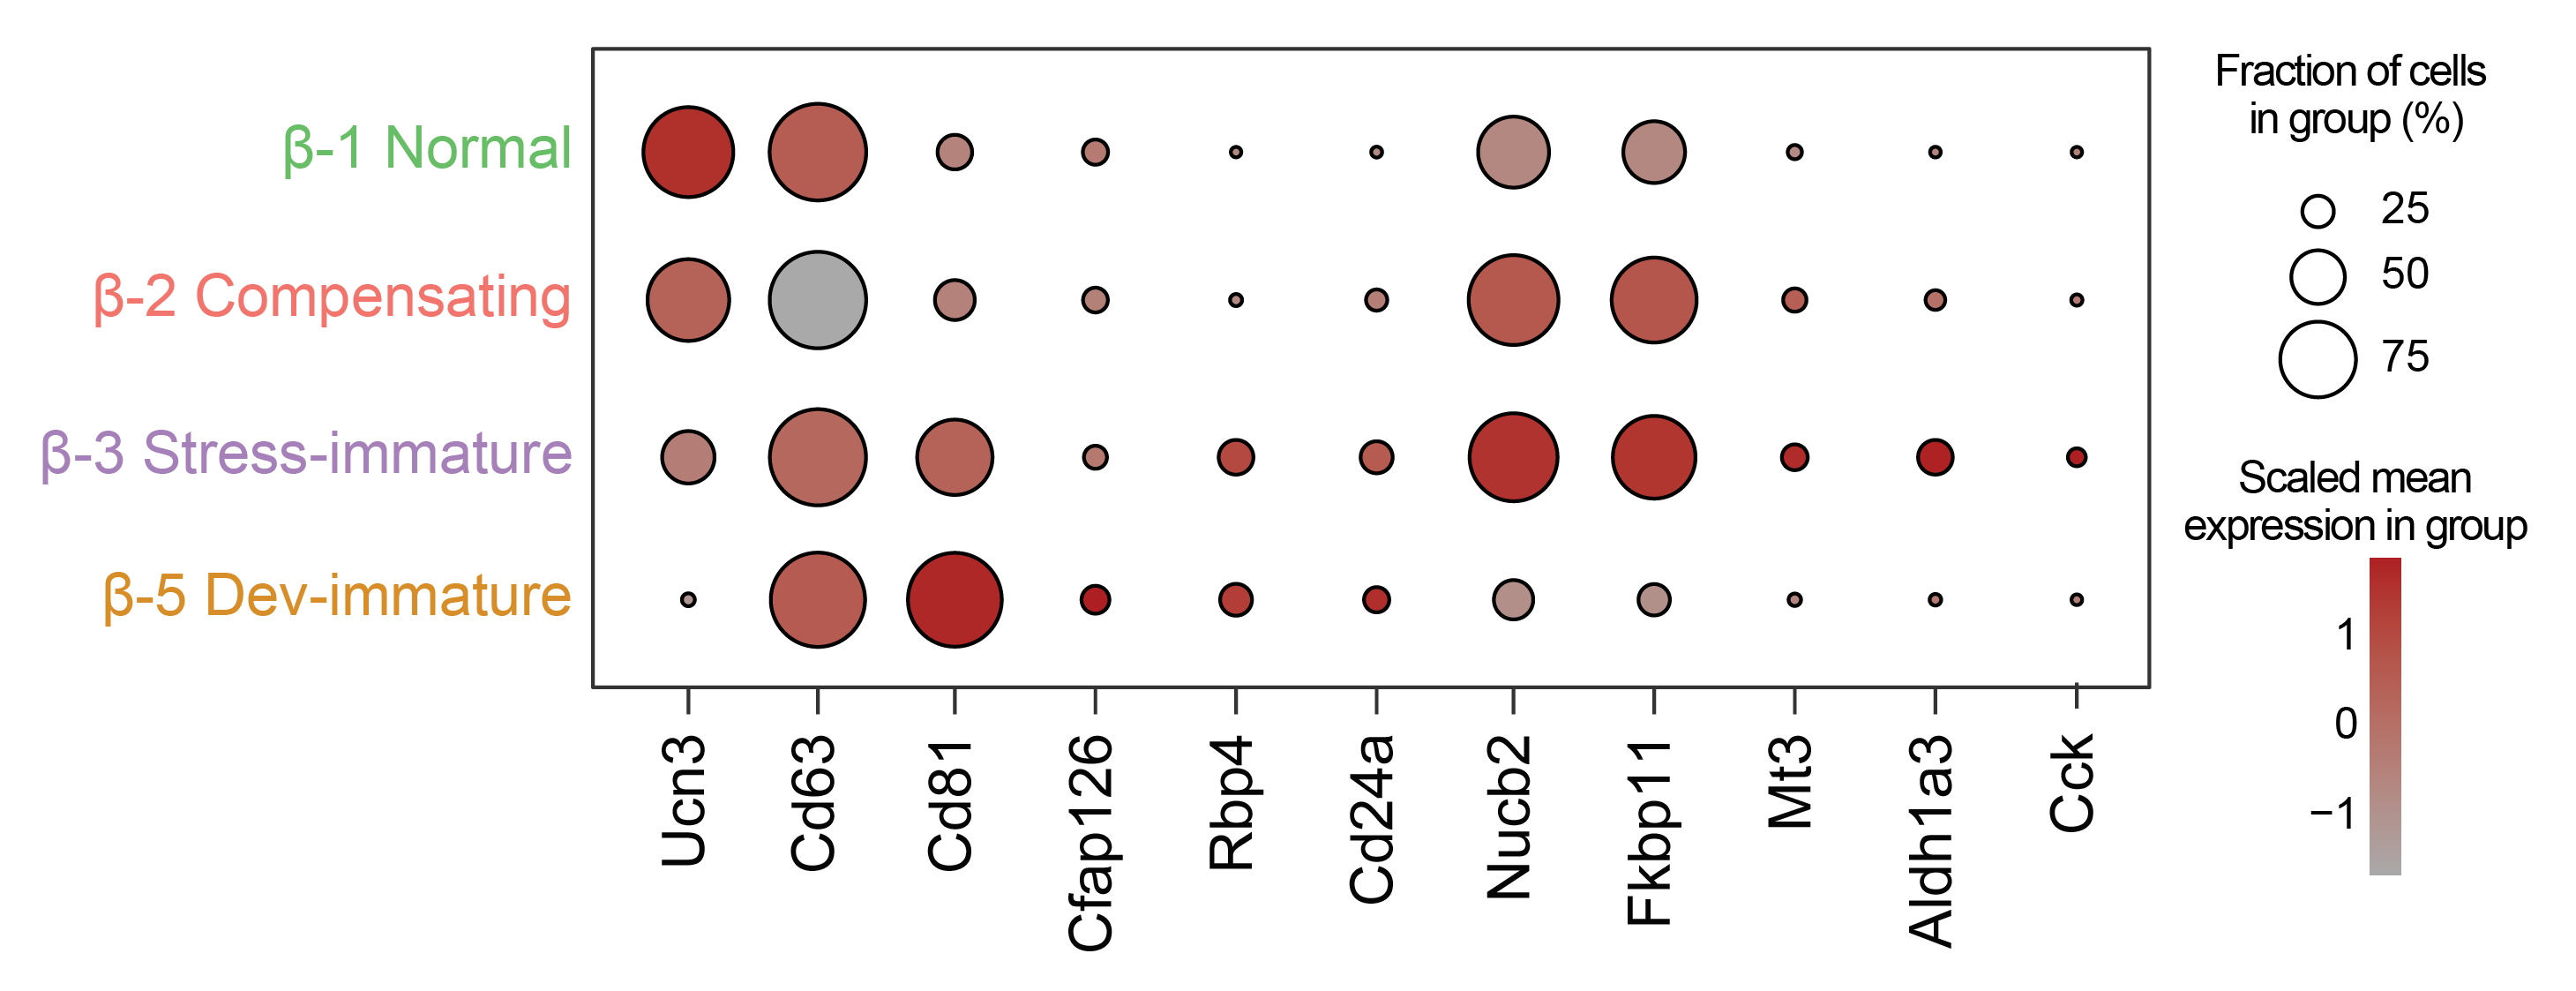
\includegraphics[width=\linewidth]{Chapter6/Fig/F3-23-01.png}
    \caption[Markers of $\beta$-cell maturity and immaturity across $\beta$-cell subsets]{\textbf{Markers of $\beta$-cell maturity and immaturity across $\beta$-cell subsets.} Dot plot depicting the expression of known markers of $\beta$-cell maturity and immaturity across $\beta$-1 normal, $\beta$-2 compensating, $\beta$-3 stress-immature and $\beta$-5 dev-immature subsets. The color of the dots represent the scaled average expression of the marker genes and the size of the dots correspond to the percentage of cells within the subset expressing the given marker gene. References: \textit{Ucn3} \textbf{\cite{blum_functional_2012}}, \textit{Cd63} \textbf{\cite{rubio-navarro_beta_2023}}, \textit{Cd81} \textbf{\cite{salinno_cd81_2021}}, \textit{Cfap126} \textbf{\cite{bader_identification_2016}}, \textit{Rbp4} \textbf{\cite{camunas-soler_patch-seq_2020}} \textit{Cd24a} \textbf{\cite{dror_epigenetic_2023}}, \textit{Nucb2, Fkbp11, Mt3}  \textbf{\cite{hrovatin_delineating_2023}}, \textit{Aldh1a3} \textbf{\cite{hrovatin_delineating_2023,kim-muller_aldehyde_2016,cinti_evidence_2016}}, \textit{Cck} \textbf{\cite{sachs_targeted_2020,chung_endocrine-exocrine_2020}}.}
    \label{fig:chp6_betacellmarkers}
\end{figure}

\par Integrating single-cell transcriptomics with functional assays and multi\textit{-omics} approaches has revolutionized our understanding of $\beta$-cell dysfunction. For instance, a study that linked single-cell transcriptomics with functional read-out via patch-clamp electrophysiology in human islet cells identified a population of RBP4\textsuperscript{+} $\beta$-cells with decreased exocytosis and significantly reduced expression of key regulators of stimulus-secretion coupling \textbf{\cite{camunas-soler_patch-seq_2020}}. Furthermore, increased levels of RBP4 are prominent in obese and \gls{t2d} individuals, and correlate with insulin resistance in the periphery. In line with these findings, we also observed high expression \textit{Rbp4} in the $\beta$-3 subset \textbf{(\autoref{fig:chp6_betacellmarkers})} which was also associated with reduced \textit{Ins1} expression \textbf{(\autoref{fig:chp3_betasubsets} B)}. Additionally, the expression \textit{Rbp4} was also high in the $\beta$-5 dev-immature subset which corresponds to its routine use as an immaturity marker \textbf{(\autoref{fig:chp6_betacellmarkers})} \textbf{\cite{camunas-soler_patch-seq_2020,salinno_cd81_2021,hrovatin_delineating_2023}}. Another single-cell multi\textit{-omics} study integrating genetic association data identified two distinct $\beta$-cell subsets in human donors, which undergo an abundance shift in \gls{t2d} triggered by reduced activity of HNF4A and HNF1A \textbf{\cite{wang_integrating_2023}}. Another single-cell multi\textit{-omics} study similarly showed HNF1A as a principal driver of intra-donor $\beta$-cell heterogeneity \textbf{\cite{weng_single_2023}}. These studies highlight the importance of  incorporating multiple modalities, such as functional assays and genetic data, to gain a more comprehensive understanding of the genetic and molecular underpinnings of $\beta$-cell dysfunction.\\

% \par  These observations parallel our findings, particularly with the $\beta$-2 Compensating subset, which is characterized by adaptive mechanisms in response to increased metabolic demands. The shift towards the $\beta$-3 Stress-immature subset under severe hyperglycemia reflects a similar decline in functional $\beta$-cell populations as observed with the reduction of CD63\textsuperscript{\textit{hi}} $\beta$-cells in diabetic conditions. Interestingly, while our analysis revealed that \glslink{mrna}{mRNA} expression of \textit{Cd63} was higher in the $\beta$-1 Normal and $\beta$-3 Stress-immature subsets compared to the $\beta$-2 Compensating subset, it is important to note that \glslink{mrna}{mRNA} expression is not always a reliable predictor of protein expression in single cells \boldlink{https://doi.org/10.1038/s42003-021-02142-w}. 

\par Collectively, while there seems to some level of overlap in findings related to $\beta$-cell heterogeneity and $\beta$-cell dysfunction across studies, discrepancies still exist. Further investigation is required to clarify the proposed compensating or intermediate state. While we were unable to ascertain any characteristic markers for this state, it is plausible that this state is regulated at a level that is not captured by single-cell transcriptomics. For example, multiple epigenetic mechanisms governing  $\beta$-cell adaptations to insulin resistance could become overwhelmed in \gls{t2d} \textbf{\cite{kim_epigenetics_2020}}. Furthermore, the activation of progenitor and immature $\beta$-cell programs, both of which are consistent with the notion of dedifferentiation and loss of function in $\beta$-cells, is linked to chromatin-associated transcriptional dysregulation in mouse and human \gls{t2d} \textbf{\cite{lu_polycomb-dependent_2018}}. Thus, future studies employing multi\textit{-omics} approaches should provide further insight about the adaptive and maladaptive programs in response to increased workloads in $\beta$-cells. One example of such multi-modal study involves the identification of two major $\beta$-cell subtypes ($\beta$\textsubscript{HI} and $\beta$\textsubscript{LO}) based on histone mark heterogeneity, which can be \gls{facs} separated into CD24\textsuperscript{+} and CD24\textsuperscript{-} fractions \textbf{\cite{dror_epigenetic_2023}}. We observed a higher expression of the CD24 mouse gene, \textit{Cd24a}, in the $\beta$-3 stress-immature subset \textbf{(\autoref{fig:chp6_betacellmarkers})} which is enriched during metabolic stress response under conditions of severe hyperglycemia \textbf{(\autoref{fig:chp3_betasubsets} D)}. Interestingly, the authors also depicted an increase in relative number of CD24\textsuperscript{+} $\beta$\textsubscript{HI} cells upon chronic \gls{hfd} feeding and also their enrichment in human \gls{t2d}. Similar multi-modal studies in the future could help elucidate the role of compensating or intermediate states in $\beta$-cell adaptation and dysfunction in \gls{t2d}.\\ 

\par While we are documenting various $\beta$-cell states in mouse models, it is important to note that we are not capturing the potential contributions of genetic background that are known to influence susceptibility to human \gls{t2d} \textbf{\cite{cauchi_genetic_2008,grarup_genetic_2014,karaderi_insights_2015,prasad_genetics_2015,wang_genetic_2016}}. It is also possible that certain sub-populations of $\beta$-cells are more predisposed to diabetes than others. This could, for example, explain how non-obese individuals can develop \gls{t2d} \textbf{\cite{vaag_non-obese_2007,olaogun_pathophysiology_2020}}. Additionally, individuals could have intrinsic differences in $\beta$-cell composition, which could affect their susceptibility to developing the disease and individuals with \gls{t2d} likely exhibit a different composition of $\beta$-cell states and/or subsets, with each subset potentially responding differently to \gls{t2d} treatments \textbf{\cite{wang_integrating_2023}}. With sophisticated lineage tracing experiments in animal models, live-cell imaging and patch-clamping techniques, we should be able to discriminate between various $\beta$-cell states and characterize their functional responses under different conditions. A prerequisite for these advanced studies is the identification of markers to better separate the various sub-populations. While this is no easy task, employing single-cell multi\textit{-omics}, extensive longitudinal studies, functional genomics screens such as \glsentryshort{crispr}-Cas9 knockout, or even an atlas approach such as ours and \gls{mia} with additional datasets can uncover a more detailed and accurate profile of the various $\beta$-cell sub-populations. Another interesting investigation would involve examining the distribution or localization of these sub-populations within the pancreas. Integrating existing data with spatial technologies such as \gls{st} \textbf{\cite{tian_expanding_2023, olaniru_single-cell_2023}} or \gls{imc} will provide in-depth mapping of these sub-populations.\\

\par This is an exciting time for the field of $\beta$-cell heterogeneity research as decades of research are gradually converging to paint a clearer picture of why and how $\beta$-cells differ. It is important to expand this research into additional preclinical models and human tissues, as heterogeneity within human islets may differ from animal models. Ultimately, it remains to be seen to what extent these findings of $\beta$-cell heterogeneity and dysfunction might lead to clinically relevant advances in diabetes therapy.


% Although, the \glslink{mrna}{mRNA} expression of \textit{Cd63} was higher in the $\beta$-1 and $\beta$-3 subsets compared to $\beta$-2, \glslink{mrna}{mRNA} expression is a poor predictor of protein expression in single cells % The study detected heterogeneity among human $\beta$-cells and identified several states with varying degrees of insulin production and \gls{upr} activation. The high insulin/low \gls{upr} state represented a state of active production, The extremely high insulin producing $\beta$-cells are likely to become stressed %The various mouse models, although differing in their ..., 

% \clearpage

\subsection[Single-Cell Transcriptomics: Navigating the Promises and Pitfalls]{Single-Cell Transcriptomics:\\Navigating the Promises and Pitfalls}
\vspace{20pt}

\par From the very first study of very few mouse primordial germ cells \textbf{\cite{tang_mrna-seq_2009}}, the field of single-cell transcriptomics has advanced significantly in a relatively short time-span. This progress is driven by methodological and technological advances, reduced sequencing costs, the rapid development of novel computational methods and tools, and widespread adoption in various areas of biological research. These advancements have enabled detailed insights into cellular heterogeneity which is a key component of biological complexity, positioning \acrfull{scr} as a truly transformative methodological advancement \textbf{\cite{noauthor_focus_2023}}.\\

\par The work presented in \textbf{\autoref{chp:diet_aging}} of this thesis highlights the significant potential of single-cell transcriptomics in elucidating the cellular diversity within mouse pancreatic islets. The ability to resolve diverse CD45\textsuperscript{+} (\textit{Ptprc}) immune cell types as well as the various CD45\textsuperscript{-} hormone-secreting endocrine cell types from mixed cell populations exemplifies the cellular resolution routinely achieved by \gls{scr} with standard analysis and annotation pipelines. We took advantage of the \gls{scr} capability to perform detailed functional annotations of the various sub-populations of macrophages and T-cells based on the expression of characteristic marker genes. Moreover, with \gls{scr}, we were able to infer compositional shifts of pro-inflammatory macrophage and cytotoxic T-cell sub-populations, which were previously challenging and limited. Additionally, the ability to infer putative \gls{lri} that likely perpetuate islet inflammation during metabolic stress with \gls{scr} enables the formulation of biological hypotheses for subsequent experimental evaluation.\\

% In models of metabolic stress, such as those induced by overnutrition and aging, our profiling efforts revealed a notable enrichment of pro-inflammatory macrophage and cytotoxic T-cell sub-populations. Such inferences on compositional shifts across experimental conditions, which were previously challenging and limited, are now feasible.  % We took advantage of this capability to annotate the various sub-populations of macrophages and T-cells  The true power of \gls{scr} was exemplified by the detailed functional annotations of the various sub-populations of macrophages and T-cells based on the expression of characteristic marker genes. Moreover, in models of metabolic stress, such as those induced by overnutrition and aging, our profiling efforts revealed a notable enrichment of pro-inflammatory macrophage and cytotoxic T-cell sub-populations. Such inferences on compositional shifts across experimental conditions were significantly more challenging and certainly limited. We were also able to infer putative \gls{lri} that likely perpetuate islet inflammation during metabolic stress. The capability to infer cell-cell interactions on a transcriptomic level from single-cell datasets enables the formulation of biological hypotheses that can subsequently be experimentally evaluated.\\

% \par Additionally, the potential of reference atlases and, reference mapping algorithms and workflows for single-cell analysis was profoundly exemplified in this thesis work. We effectively showcased the integration of multiple \gls{scr} datasets to form a comprehensive $\beta$-cell reference atlas. The integrated atlas allowed for a more accurate and unified interpretation of $\beta$-cell states across various experimental conditions, enabled the comparison of cell-state shifts across studies and contextualize disease states within a healthy reference framework. Importantly, we demonstrated the application of label transfer workflows to re-annotate $\beta$-cells from external studies thereby exemplifying automated annotation to facilitate the analysis of new or the re-analysis of existing datasets. 

\par Additionally, this thesis exemplified the potential of reference atlases and mapping algorithms for single-cell analysis by integrating multiple \gls{scr} datasets to create a comprehensive $\beta$-cell atlas. This atlas enabled an unified interpretation of $\beta$-cell states across experimental conditions, facilitated cross-study comparisons, and relate them to states observed during homeostasis. Importantly, we demonstrated automated annotation using label transfer workflows to re-annotate $\beta$-cells from external studies. Such reference atlases significantly enhance the scale and generalizability of single-cell analyses, marking a substantial step towards consensus-based cell type annotations. As reference mapping evolves, it is surely poised to replace unsupervised clustering and manual annotation workflows. This transition will become increasingly feasible as more reference atlases for individual tissues in humans, mouse and other model organisms across multiple modalities become available. While there are several obstacles to be addressed, for example, logistical and computational challenges, the quality of the datasets that constitute the atlas and the underlying reference mapping algorithms, and the lack of systematic approaches towards harmonizing cell-type terminology and annotation depth, these large-scale datasets and methods will enhance future single-cell analyses, advancing our understanding of cellular heterogeneity and the pathogenesis of various diseases \textbf{\cite{lotfollahi_mapping_2021,lotfollahi_future_2024}}.\\ 

% Furthermore, this hinders our ability to study transcript isoform diversity, allele-specific expression, and post-transcriptional RNA modifications, which require full transcript sequence information. by providing insights into dynamic transitions of $\beta$-cell states and infer the speed and trajectory of $\beta$-cell dysfunction in response to chronic metabolic stress.the analysis of   In the study of \gls{t2d} pathogenesis, much attention has been devoted to the pivotal role of $\beta$-cells in regulating glucose homeostasis. However, can provide insights into the changes that underline maladaptive responses within the islets beyond the insulin-centric view, 

% \par Single-cell methodologies, including \gls{scr}, generate significant technical noise due to the small amount of material being measured. This noise can result from various sources, including stochastic gene expression and variability in \glslink{rna}{RNA} capture efficiency. Additionally, biases or artefacts can be introduced at every step of a single-cell experimental protocol, from tissue dissociation, cell isolation and lysis to reverse transcription and library preparation. This could affect downstream analysis steps and overall interpretation of the data. Moreover, batch effects are one of the most common issues in single-cell experiments. Batch effects occur due to variations in sample handling, reagent batches, and sequencing runs, which can confound biological signals. Thus, efficient sample preparation is an essential pre-requisite for any single-cell study. This involves not only the technical aspects of cell handling and processing but also the planning of experimental design to ensure reproducibility and reliability. While, rigorous quality control measures and computational analyses play a critical role in addressing the limitations and artefacts in single-cell transcriptomics data, it is important to recognize that they might not completely eliminate all biases and artefacts. For instance, batch-correction methods can over-correct to the extent that true biological signals might be lost. Therefore, it is crucial to integrate biological knowledge with computational analyses to ensure the accuracy and relevance of conclusions drawn from the data. 

% An optimal quality sample is an essential pre-requisite for any single-cell study. Complex tissues, such as pancreas, require specific tissue dissociation methods and islet isolation protocols. Tissue dissociation and cell isolation, which represent a crucial step in sample preparation, can cause physical stress to cells, altering their transcriptional state \boldlink{https://doi.org/10.15252/msb.202211147} or leading to cell damage or death. This is particularly important for fragile cell-types that may not survive the isolation process, resulting in their under-representation or loss. Furthermore, the isolation of islets from the surrounding exocrine tissue is not straightforward and several factors such as the digestion enzyme and islet purification steps must be carefully considered. Furthermore, during the cell isolation and the downstream encapsulation step 

%  The greatest source of unwanted technical artefacts in any single-cell study arguably is the single-cell preparation protocols themselves, and therefore require careful optimization so as to introduce the least artifact.  For \textit{e.g.}, the variation demonstrated by \gls{scr} in isolated macrophages might not reflect \textit{in vivo} biology, as tissue dissociation recovers only a small proportion of tissue-resident macrophages and the single-cell protocols may activate macrophages during isolation steps \boldlink{https://www.sciencedirect.com/science/article/pii/S0006497123020190}

% \par Single-cell transcriptomics, while transformative, inherently carries several limitations that must be carefully considered when evaluating findings from this thesis or any study employing this technology. For instance, the 10x Chromium 3' v3 Gene Expression protocol employed in this thesis introduces a 3' bias where sequences near the 3' end of the transcript are preferentially captured and sequenced, thereby affecting all genes \textbf{\cite{mawla_navigating_2019}}. Such methodologies generate substantial technical noise from various sources, including stochastic gene expression and variability in RNA capture efficiency. Additionally, biases and artifacts can be introduced at every procedural step—from tissue dissociation to library preparation—potentially skewing the data interpretation \boldlink{https://doi.org/10.3389/fcell.2018.00108}. Compounding these are batch effects, common in single-cell experiments, caused by variations in sample handling and sequencing that can obscure biological signals \textbf{\cite{heumos_best_2023}}. Importantly, individual cells cannot contribute as much as information as bulk samples due to the sparse nature of \gls{scr} data. In addition to rigorous \gls{qc} measures and computational efforts to address these artifacts, it is crucial to integrate biological knowledge with computational analyses to ensure the accuracy and relevance of conclusions drawn from the data. Despite the widespread adoption of \gls{scr}, overall experimental costs remain high even as if the cost per cell is decreasing. Therefore, the choice of the experimental approach should be dictated by the experimental questions in order to perform more accurate and cost-effective studies. Overall, continued advancements in experimental design, technical limitations and computational methods are essential to overcome these challenges and refine the reliability of single-cell studies.Thus, efficient sample preparation is an essential pre-requisite for any single-cell study. This involves not only the technical aspects of cell handling and processing but also the planning of experimental design to ensure reproducibility and reliability. Importantly, individual cells cannot contribute as much as information as bulk samples due to the sparse nature of \gls{scr} data

\par However, single-cell transcriptomics inherently carries several limitations that must be carefully considered when evaluating findings from this thesis or any study employing this technology. An optimal quality sample is an essential prerequisite for any single-cell study. Complex tissues, such as pancreas, require specific tissue dissociation methods and islet isolation protocols. Tissue dissociation and cell isolation, which represent a crucial step in sample preparation, can cause physical stress to cells, altering their transcriptional state or leading to cell damage or death \textbf{\cite{neuschulz_singlecell_2023}} . This is particularly important for fragile cell-types that may not survive the isolation process, resulting in their under-representation or loss. Furthermore, the isolation of islets from the surrounding exocrine tissue is not straightforward and several factors such as the digestion enzyme and islet purification steps must be carefully considered. The greatest source of unwanted technical artefacts in any single-cell study arguably is the single-cell preparation protocols themselves, and therefore require careful optimization so as to minimize artefacts and batch effects. Additionally, the choice of experimental protocol in itself is a considerable source of bias. For instance, the 10x Chromium 3' v3 Gene Expression protocol employed in this thesis introduces a 3' bias where sequences near the 3' end of the transcript are preferentially captured and sequenced, thereby affecting all genes \textbf{\cite{mawla_navigating_2019}}. While not the focus of this work, 3' sequencing hinders our ability to study transcript isoform diversity, allele-specific expression, and post-transcriptional \glslink{rna}{RNA} modifications, all of which require full transcript sequence information.\\

% These methodologies generate significant technical noise due to the small amount of material being measured. This noise can result from various sources, including stochastic gene expression and variability in \glslink{rna}{RNA} capture efficiency. Additionally, biases or artefacts can be introduced at every step of a single-cell experimental protocol, from tissue dissociation, cell isolation and lysis to reverse transcription and library preparation \boldlink{https://doi.org/10.3389/fcell.2018.00108}. This could affect downstream analysis steps and overall interpretation of the data. \\ individual cells cannot contribute as much as information as bulk samples due to the sparse nature of \gls{scr} data

\par Importantly, analysis of individual cells is limited by dropout effects for lowly expressed genes that are better captured in bulk approaches \textbf{\cite{kharchenko_triumphs_2021}}. Moreover, batch effects are one of the most common issues in single-cell experiments and occur due to variations in sample handling, reagent batches, and sequencing runs, which can confound biological signals \textbf{\cite{heumos_best_2023}}. Additionally, biological factors such as cell size and cell cycle state could play important roles in cell variability for certain cell types and could affect downstream clustering approaches \textbf{\cite{chen_single-cell_2019}}. Unsupervised and even supervised clustering algorithms represent one of the most important components of single-cell analysis as most downstream tasks are carried out based on clusters. Consequently, the final conclusions can be significantly influenced by the clustering step. It is important to recognize that not all obtained clusters may be biologically meaningful; clustering algorithms can inadvertently partition random noise into clusters, which may obscure or distort the true biological variability \textbf{\cite{kiselev_challenges_2019}}. Thus, rigorous \gls{qc} measures, preprocessing and downstream computational analyses play a critical role in addressing the limitations and artefacts in single-cell transcriptomics data. However, it is important to recognize that they might not completely eliminate all biases and artefacts. For instance, batch-correction methods can over-correct to the extent that true biological signals might be lost \textbf{\cite{luecken_benchmarking_2021}}. Therefore, it is crucial to always integrate biological knowledge with computational steps to ensure the accuracy and relevance of conclusions drawn from the data.\\

\par Looking ahead, ongoing advancements in study design, sample processing, and computational methods, \gls{scr} and other single-cell \textit{-omics} methods will likely continue to expand their already substantial roles in biomedical research. Such progress will enable these technologies to ultimately realize their promise of leading to an understanding of the function of an individual cell in the context of varying microenvironments associated with changing physiology and disease states \textbf{\cite{eberwine_promise_2014}}.

% \par Thus, the choice of experimental approach should be dictated by the research question. In certain cases, a bulk transcriptome approach might be more beneficial in spite of the perceived novelty of \gls{scr}. Conversely, when transcriptional heterogeneity is the central focus, \gls{scr} might be the only choice. Even in these cases, the findings must be subjected to extensive validations using independent approaches. Overall, aided by continued advancements in experimental design, technical limitations and computational methods, \gls{scr} and other single-cell \textit{-omics} methods will remain as main stays in 


\clearpage


\subsection[From Rodents to Humans: Bridging the Gap in \glsentryshort{t2d} Research]{From Rodents to Humans:\\Bridging the Gap in \gls{t2d} Research}
\vspace{20pt}
\par The wide availability of pancreatic tissue from \gls{t2d} and non-diabetic individuals has greatly facilitated the comparative analysis of \gls{t2d} $\beta$-cells. Several modalities have enabled the in-depth characterization of  the functional, molecular and metabolic features of \gls{t2d} $\beta$-cells \textbf{\cite{avrahami_single-cell_2020,camunas-soler_patch-seq_2020,cohrs_dysfunction_2020,wigger_multi-omics_2021,gloyn_every_2022}}. However, studying \gls{t2d} in humans presents significant challenges, such as variability in disease progression and treatment among patients, ethical considerations that limit experimental interventions and the influence of genetic and environmental factors that complicate the interpretation of results \textbf{\cite{haga_ethical_2009,prasad_genetics_2015}}. As a result, these challenges necessitate the reliance on various animal models,particularly mouse models, which have been indispensable in this thesis work for dissecting the complex cellular and molecular mechanisms underlying \gls{t2d}.\\

% employed the C57BL/6 strain of mice which are the most sensitive to diet-induced obesity and develop severe obesity, increased glucose intolerance, moderate insulin resistance and elevated glucose levels in response to western diets, including \gls{hfd}s.\\ \begin{itemize}
%     \item  - 12-week-old C57BL/6J mice homozygous for the obese (ob) mutation in the leptin gene (\textit{Lep}) from Chung \textit{et al.} \textbf{\cite{chung_endocrine-exocrine_2020}} \textit{and}
%     \item  - 6-week-old and 9-week-old mixed strain mice homozygous for the diabetes (db) mutation in the leptin receptor (\textit{Lepr})
% \end{itemize}

\par The \gls{wd} feeding model facilitated the study of diet-induced obesity and metabolic stress, and in particular, inflammation of the pancreatic tissue, which has relevance to human obesity and mirrors dietary influences on human diabetes. On the other hand, the aging model under standard chow diet underscored the natural progression of metabolic dysfunction and systemic inflammation associated with aging. Therefore, both the diet-induced obesity and the aging models are appropriate for studying pre-diabetes or diabetes-related metabolic syndrome as opposed to severe disease \textbf{\cite{the_jackson_laboratory_choosing_nodate}}. The genetic mice models included in this thesis work (C57BL/6J \textit{Lep\textsuperscript{ob}} mice and mixed strain \textit{Lepr\textsuperscript{db}} mice) are the most popular animal models in \gls{t2d} research. Both models exhibit phenotypes, characteristic of human \gls{t2d} - obesity induced by unregulated feeding, severe insulin resistance and hyperglycemia \textbf{\cite{the_jackson_laboratory_choosing_nodate}}. The observed phenotypic differences between the \textit{db/db} model utilized here and the \textit{ob/ob} model employed in \textbf{\cite{chung_advances_2021}} likely stem from the differences in the age of mice and the background strain, as mixed strains are typically more disease resistant compared to pure strains \textbf{\cite{birchler_unraveling_2006}}.\\

\par Apart from genetically modified mouse strains, chemically induced \gls{t2d} models also offer valuable insights into mechanisms underlying $\beta$-cell failure. The partial $\beta$-cell ablation model using \gls{stz} by Sachs \textit{et al.} \textbf{\cite{sachs_targeted_2020}} shed light on maladaptive processes in $\beta$-cells upon reduction of their mass, which reflects situations of $\beta$-cell loss in humans \textbf{\cite{prentki_islet_2006}}. The use of S961, an insulin receptor antagonist, to model impairment in the insulin receptor signaling and insulin mediated effects, which are key features of \gls{t2d}, offered an unique perspective on $\beta$-cell workload under severe hyperglycemia without the confounding effects of $\beta$-cell loss or obesity \textbf{\cite{vikram_inhibition_2011}}.\\

\par Collectively, the mouse models represented in this work allowed for a comprehensive exploration of \gls{t2d} pathogenesis, and revealed the heterogeneity and dynamic responses of $\beta$-cells and immune cells in response to various stressors. More importantly, this thesis further underscores the utility of rodent models in providing detailed molecular insights that may prove crucial for developing targeted therapies. By leveraging the strengths of each mouse model, critical advances in diabetes research can pave the way for more effective therapeutic strategies. It is important to note here that most of the mouse models discussed as part of this thesis work used male mice, as male rodents, in general, are more susceptible to obesity, insulin resistance and glucose intolerance compared to female rodents \textbf{\cite{lutz_mammalian_2023}}. Additionally, the exclusion of female rodents can also be to avoid complications with the estrous cycle \textbf{\cite{stott_high_2020}}. Future studies should make every possible effort to include male and female counterparts in any form of diabetes research to enhance our understanding of \gls{t2d} in both sexes and its associated phenotypes as well as better characterize the differences in \gls{t2d} phenotypes between males and females.\\

\par As anyone would expect, the mouse models specifically utilized in this thesis work and additionally included from external studies represent a small fraction of the plethora of animal models available for \gls{t2d} research. Besides mice as a rodent model, rats are also regularly used to model \gls{t2d} and facilitate certain experimental procedures due to their larger size than mice. Among the several rat models, the Zucker Diabetic Sprague-Dawley rat combines insulin resistance with $\beta$-cell defects \textbf{\cite{peterson_characterization_2015,lutz_mammalian_2023}}. Several rodent models transgenic for \gls{hiapp} have revealed the effects of \gls{hiapp} on $\beta$-cell apoptosis in \gls{t2d}. Since rodent \gls{iapp} is not amyloidogenic, these transgenic rodent models provide an opportunity to elucidate the mechanisms responsible for hIAPP-induced $\beta$-cell apoptosis while circumventing species differences between rodents and humans \textbf{\cite{matveyenko_islet_2006,hoppener_human_2008}}.\\


\par Besides rodent models, large animal models including pigs, sheep, dogs, cats and rabbits are frequently used in diabetes research \textbf{\cite{cefalu_animal_2006,lutz_mammalian_2023,singh_animal_2024,covington_animal_2024}}. Among all the animal models, the presentation of \gls{t2d}-like disease in non-human primates most closely represents the metabolic phenotype characteristic of human \gls{t2d} \textbf{\cite{lutz_mammalian_2023,cefalu_animal_2006}}. The diabetic rhesus monkey, for example, closely mimics human \gls{t2d} in terms of disease progression and complications (\textit{e.g.} atherosclerosis), making the model extremely valuable for translational studies \textbf{\cite{singh_animal_2024}}. In recent years, islet organoid models, derived from human tissue cells or pluripotent stem cells, are emerging as additional tools in the the study of pancreatic cell development, physiology, action of pancreatic hormones on target tissues and for functional and screening assays \textbf{\cite{beydag-tasoz_towards_2023,zhang_islet_2022}}.\\

\par While critical advances in biomedical research have been made using animal models, they also present obstacles. The failures in downstream drug discovery workflows are often blamed on poor quality animal models \textbf{\cite{mcmurray_mouse_2011}}. Even with well-designed and carefully executed studies involving animal models, challenges remain. As an example that is relevant in the context of this thesis - in a systematic comparison of the inflammatory responses between human and mouse models, Seok \textit{et al.} demonstrated dramatic difference in gene expression profiles associated with inflammation between mice and humans, while noting several disparities between the two species that could likely contribute to the observed differences \textbf{\cite{bolker_animal_2017, seok_genomic_2013}}. In this thesis, we performed the \gls{go} analysis in \textbf{\autoref{sec:chp2_sc_macs}} and \textbf{\autoref{sec:chp2_sc_macs3_diff}} by directly comparing mouse genes against human gene sets and in case of cell-cell interactions analysis in \textbf{\autoref{sec:chp2_cell_cell}}, we first converted mouse genes to human genes in order to utilize \glspl{lri} curated for humans in CellChat. While these analyses were set up in such manner in order to gain human context and potentially enhance the relevance of our research to human biology, this approach also presents certain limitations. Directly comparing mouse genes to human gene sets in the \gls{go} analysis may yield less accurate results. Similarly, using human orthologs of mouse genes may introduce discrepancies as biological functions and interactions of these genes can differ between mice and humans. These methodological choices underscore the inherent challenges in using animal models to recapitulate human disease contexts. Reliable inferences from animal models requires careful consideration of the evolutionary history between the species.\\

\par Even if we keep the species disparities aside, no single animal model can fully mimic the complex pathophysiological processes involved in \gls{t2d} \textbf{\cite{singh_animal_2024}}. This could also, in part, be attributed to the controlled and well-regulated environments in which model animals are housed and the genetic homogeneity amongst them \textbf{\cite{bolker_animal_2017}}. \gls{t2d} is caused by combination of environmental factors and there is considerable heterogeneity in both pathology and treatment responses in patients. To address these limitations, it is of utmost importance to incorporate a wider range of animal models and varying experimental conditions as well as integrate human-derived data to gain a more comprehensive understanding of \gls{t2d}. There is no straight-forward answer for which animal model to choose as there is no `perfect' model available for \gls{t2d}. Despite these limitations, mice and other animal models will remain vital tools for experimental studies related to pathogenic mechanisms in \gls{t2d}. Instead, the choice should be guided by specific research questions and the aspect of the disease being investigated. Factors such as genetic background, physiological relevance to a process in human disease, and the specific conditions being modeled are crucial in determining the appropriate model system. In this way, researchers can ensure that their findings are relevant and can be translated to humans, thereby paving the way for more effective therapies for \gls{t2d}.

\subsection[Implications on therapeutic strategies for \glsentryshort{t2d}]{Implications on therapeutic strategies for \gls{t2d}}

\par One of the most impactful medical achievements of the 20\textsuperscript{th} century was the discovery of insulin by Frederick G. Banting and his colleagues. This discovery changed the landscape of diabetes care forever. Over the past century, numerous landmark achievements have propelled rapid innovations and advancements in clinical management of diabetes. As we transition into the next century of diabetes research, several critical questions remain unanswered, presenting abundant opportunities for further exploration and addressing unmet medical needs in diabetes care \textbf{\cite{cefalu_heterogeneity_2021}}. \\    

\par The current worsening epidemic of \gls{t2d} affects millions worldwide, thereby necessitating effective management strategies. The management of \gls{t2d} typically involves a combination of lifestyle modifications— healthy diet, increased physical activity, self-monitoring of glucose levels, and maintaining a healthy weight, with pharmacological interventions. A significant palette of anti-diabetic drugs are available which include insulin secretagogues (sulfonylureas and meglitinides), biguanides like metformin, and insulin sensitizers such as thiazolidinediones. Newer drug classes include \gls{glp1ra} and \gls{dpp4i}, which enhance insulin secretion and incretin hormone activity, as well as \gls{sglt2i} \textbf{\cite{padhi_type_2020}}. \gls{glp1ra}s, in particular, enable weight loss and induce insulin sensitization in peripheral tissues, which impacts feeding in addition to its effects on $\beta$-cells. Despite these advancements, the progressive nature of \gls{t2d} often necessitates insulin therapy, which further improves glycemic control but at the risk of hypoglycemia. Additionally, surgical interventions such as bariatric surgery have shown significant benefits in improving glycemic control and inducing remission in some patients with \gls{t2d} \textbf{\cite{schauer_philip_r_bariatric_2014,schauer_philip_r_bariatric_2017,oppenlander_vertical_2021}}.\\

% \textbf{\cite{bloemendaal_effects_2014,yaribeygi_molecular_2019}}

% Recent innovations, like the fully-closed loop insulin delivery system (artificial pancreas), demonstrate promising improvements in glycemic control by automatically modulating insulin delivery based on continuous glucose monitoring \textbf{\cite{daly_fully_2023}}.\\

% \par The current worsening epidemic of \gls{t2d} is affecting the life and health of humans all around the world. The management of \gls{t2d} typically involves a combination of lifestyle modifications and pharmacological treatments aimed at controlling blood glucose levels and improving insulin sensitivity. The first intervention strategy involves adoption of an overall healthier lifestyle, with healthy diet, increased physical activity, self-monitoring of plasma glucose levels and maintaining a healthy body weight. A significant palette of anti-diabetic drugs are available which include insulin secretagogues (sulfonylureas and metiglinides) that increase insulin secretion, biguanides such as metformin which improves body's response to natural insulin and reduces hepatic glucose output, and insulin sensitizers such as thiazolidinedione, also known as glitazones, which increases the insulin sensitivity in muscle, liver and adipocytes. Newer classes of drugs for \gls{t2d} include incretin mimetics such as \glslink{glp1}{GLP-1} agonists (GLP-1A) or \glslink{glp1}{GLP-1} receptor agonists (GLP-1RA) and dipeptidyl peptidase 4 (DPP-4) inhibitors. The \glslink{glp1}{GLP-1}RA agonists are injectable medications which the incretin hormone \glslink{glp1}{GLP-1}, which increases insulin secretion, decreases glucagon secretion, slows gastric emptying, and induces satiety. They can also promote weight loss which have led to their recent surge in popularity. DPP-4 inhibitors on the other hand increase the levels of \glslink{glp1}{GLP-1} by inhibiting its degradation. Another example in newer class of drugs are the sodium-glucose co-transporter 2 (SGLT2) inhibitors, which reduce renal glucose re-absorption, increasing urinary glucose excretion, and provide potential cardiovascular and renal benefits. However, the progressive nature of \gls{t2d} mandates the initiation of insulin therapy which further improves glycemic control but at the risk of hypoglycemia. In a recent study, researchers demonstrated a fully-closed loop insulin delivery system (artificial pancreas) which comprises a continuous glucose monitor, an insulin pump and a control algorithm that automatically modulates subcutaneous insulin delivery, as a safe and effective approach to improve glycemic control in people with \gls{t2d} \boldlink{https://doi.org/10.1038/s41591-022-02144-z}.\\

\par However, current pharmacological treatments do not halt the decline of $\beta$-cell function, which is a hallmark of \gls{t2d} . There is evidence to suggest that intensive insulin therapy at disease onset prevents $\beta$-cell exhaustion and better preserves $\beta$-cell function compared to oral anti-diabetic drugs \textbf{\cite{wysham_beta-cell_2020}}. The deterioration of $\beta$-cell function is likely an important cause in the failure of several anti-hyperglycemic therapies. Thus, an understanding of the mechanisms of $\beta$-cell dysfunction is urgently required to stop, or even reverse disease progression and provide better therapeutic options for patients. Prioritizing the cataloging of $\beta$-cell heterogeneity at various cellular and molecular levels and leveraging this knowledge to design therapies should be a critical goal of diabetes research. This could ultimately have profound implications for the development of $\beta$-cell replacement therapies such as transplantation of new $\beta$-like cells derived from human pluripotent stem cells, harvesting islets from genetically engineered animals, stimulating endogenous $\beta$-cell proliferation, triggering the re-differentiation of dedifferentiated $\beta$-cells or the trans-differentiation of non-$\beta$-cells to $\beta$-like cells \textbf{\cite{zhou_pancreas_2018}}.\\

\par Human islet transplantation has been a successful cell-based therapy for \gls{t1d} \textbf{\cite{cefalu_heterogeneity_2021}} and studies transplanting induced pluripotent stem cells-derived insulin-producing cells in a \textit{db/db} mouse model show promise for glucose normalization \textbf{\cite{alipio_reversal_2010}}. However, challenges such as insulin resistance, immune reactions, and  dysfunction of transplanted $\beta$-like cell due to glucolipotoxicity might necessitate combination therapies to maintain the health and functionality of the transplanted cells \textbf{\cite{salib_stem_2022}}. Therapeutic approaches focused on increasing $\beta$-cell proliferation are also not sufficient in improving long-term outcomes of diabetes, further necessitating combination therapies to protect $\beta$-cells from apoptosis or dedifferentiation from diabetogenic insults in \gls{t2d} or protecting islets from activated autoreactive immune cells in \gls{t1d} \textbf{\cite{eguchi_dysregulation_2022}}. Triggering the re-differentiation of dedifferentiated $\beta$-cells is an intuitive approach as it mirrors the differentiation process of $\beta$-cells during development. The partial $\beta$-cell ablation study by Sachs \textit{et al.} revealed pharmacological entry points, particularly insulin treatment, to target dedifferentiated $\beta$-cells for diabetes remission in a mouse model \textbf{\cite{sachs_targeted_2020}}. Another study demonstrated that pair feeding in \textit{db/db} animals resulted in partial redifferentiation of $\beta$-cells, restoring the expression of insulin, Foxo1, MafA and NeuroD1, while suppressing the dedifferentiation marker, \textit{Aldh1a3} \textbf{\cite{ishida_pair_2017}}. Furthermore, preclinical and clinical data from \gls{t1d} and \gls{t2d} patients suggest a transient recovery of $\beta$-cell function upon glycemic normalization following insulin treatment, achieved either through $\beta$-cell rest or redifferentiation \textbf{\cite{harrison_-cell_2012,wang_pancreatic_2014}}. Altogether, these findings highlight the potential for innovative combination therapies to significantly enhance the effectiveness of diabetes treatments and improve patient outcomes.\\

\par Given that the chronic, low-grade inflammation of metabolic tissues, including pancreas and pancreatic islets, is now considered to be a part of the etiology of \gls{t2d} \textbf{\cite{cuenco_islet_2022}}, anti-inflammatory strategies could be helpful not only to control \gls{t2d} symptoms but also to treat its causes. Similar to re-establishing glycemic control, dietary interventions and regular physical activity can reduce the ongoing inflammatory responses in \gls{t2d}. Furthermore, the anti-diabetic drugs discussed above also exert immunomodulatory effects, including the reduction of inflammatory infiltration in peripheral tissues and pancreatic islets, along with a subsequent decrease in the synthesis of the pro-inflammatory mediators \textbf{\cite{kurylowicz_anti-inflammatory_2020}}. In addition, animal studies have depicted the potential effects of \glspl{nsaid} on glucose homeostasis, including the increase of insulin sensitivity via reduction of systemic inflammation and improvement of insulin secretion due to the anti-inflammatory effect on pancreatic islets \textbf{\cite{kurylowicz_anti-inflammatory_2020}}. Anti-cytokine therapies could also constitute as an alternative treatment targeting the inflammatory mediators. Anti-\gls{tnf}-$\alpha$ therapy has shown favorable effects on insulin resistance and \gls{t2d} risk in patients with various autoimmune diseases. Additionally, \gls{il}-1$\beta$ antagonism mitigated $\beta$-cell dysfunction and improved glycemia and cardiovascular complications. While our study highlighted a role for \gls{ifn}-$\beta$1 in islet macrophages during \gls{wd}-induced obesity and aging, another study demonstrated that overexpression of the \textit{Ifnb1} gene in \gls{hfd}-fed mice suppressed immune cell infiltration into adipose tissue and attenuated the production of pro-inflammatory cytokines. Furthermore, \gls{ifn}-$\beta$1 improved insulin sensitivity and glucose homeostasis \textbf{\cite{alsaggar_interferon_2017}}. Thus, therapies targeting \gls{ifn}-$\beta$1 might have promising potential for clinical applications in the prevention and treatment of inflammation-driven pathologies. Additionally, interventions increasing the number of \gls{treg} in diet-induced obesity models resulted in improved insulin resistance and glucose tolerance \textbf{\cite{winer_normalization_2009,feuerer_lean_2009}}. These findings suggest that enhancing T-reg populations could be a viable strategy for managing metabolic dysfunctions associated with obesity and \gls{t2d}. Ultimately, immunomodulatory drugs, either alone or in combination, could prove an effective treatment for \gls{t2d} and other associated inflammatory diseases \textbf{\cite{rohm_inflammation_2022}}. Well-designed trials will be essential to translate the findings from preclinical studies into medical practice.\\

\par Collectively, therapies such as those discussed above combined with technological advances have put us on the brink of precision or personalized medicine, which is anticipated to improve the quality of life in patients compared to standards of care available today.

% Furthermore, age-dependent differences between juvenile and adult $\beta$-cells might require use of different factors to induce expansion. , improving insulin sensitivity by restoring the insulin signaling cascade and decreasing fasting glucose in obese, non-diabetic individuals, though these findings require further verification in clinical trials. Similarly, %\par
%\end{comment}
%\clearpage

\section{Limitations and Future Work}

\par The wealth of data generated in both projects within this thesis offers several avenues for future research. For instance, advanced single-cell multi\textit{-omics} integration methods could comprehensively integrate \gls{imc} and \gls{scr} data \textbf{\cite{repapi_integration_2023}}, providing a more detailed and dynamic understanding of the immune sub-populations mediating pancreatic and islet inflammation in diet-induced obesity and aging. Subsequently, analysis methods like trajectory inference could be used to reconstruct the dynamics of the immune cell types across the pancreatic tissue. Understanding these dynamics is crucial, as it provides insights into the cellular mechanisms driving pancreatic health and disease. One key aspect of pancreatic health is the role of homeostatic macrophages, which are known to play an indispensable role in regulating $\beta$-cell health within pancreatic islets \textbf{\cite{eguchi_islet_2017}}. Future studies investigating cell-cell interactions between macrophages, $\beta$-cells and other cell types could reveal additional altered signaling pathways that cause $\beta$-cell dysfunction within inflamed islets during overnutrition and/or aging.\\


% Unlike the qualitative associations of \gls{imc} and \gls{scr}, integrating these modalities quantitatively could elucidate more precise relationships and interactions between these immune cells

\par For future studies related to \textbf{\autoref{chp:meta_analysis}}, recalculating gene expression for all the samples to include intronic counts can enable \glslink{rna}{RNA} velocity analyses, enhancing our understanding of the dynamic transitions and trajectory of $\beta$-cell dysfunction in \gls{t2d} in response to chronic metabolic stresses. This approach would enhance the ranked \gls{pc} pseudotime analysis \textbf{(\autoref{sec:chp3_betaPCA})}, offering insights into the speed and direction of $\beta$-cell state changes. Additionally, integrating \gls{grn} analysis \textbf{(\autoref{sec:chp3_betaGRN})} could link these dynamic gene expression changes to underlying regulatory circuits, thereby offering a more comprehensive view of \glspl{tf} and pathways driving $\beta$-cell responses in \gls{t2d}. Beyond $\beta$-cells, the islet non-$\beta$-cells such as $\alpha$-cells, $\delta$-cells and PP-cells are also important components of islet architecture and intercellular communication. Emerging evidence points to the deterioration of $\alpha$-cell and $\delta$-cell function in diabetes \textbf{\cite{brereton_alpha-_2015,gao_-cells_2021,brooks_not_2023}}. Future analysis of the available single-cell data for the non-$\beta$-cells in the islet could characterize broader islet defects, shifting the focus from solely insulin-centric to include maladaptive responses in other islet cell types, and address the complex paracrine interplay contributing to metabolic dysfunction in \gls{t2d}.\\

\par While experimental validation would be beyond the scope of this thesis, future validation studies to confirm the accuracy of the observed results and exploration of the predictions made are a possible avenue to follow up on this thesis work.

\clearpage

\section{Concluding Remarks}
\vspace{-5pt}
\par This thesis work sheds light on complex mechanisms underlying \glsentrylong{t2d} (\gls{t2d}), particularly focusing on the role of pancreatic inflammation and islet $\beta$-cell dysfunction. With multi-parametric, single-cell approaches, we highlighted the pivotal role of CD45\textsuperscript{+} immune cells dynamics and $\beta$-cell heterogeneity under metabolic stresses.\\

\par  In \textbf{\autoref{chp:diet_aging}}, we utilized a multi\textit{-omics} approach to identify immune cell sub-populations within pancreatic tissue and islets, revealing a pro-inflammatory macrophage sub-population that responded differently to overnutrition and aging. Through cytokine-mediated cellular communication, this macrophage sub-population may talk to CD8\textsuperscript{+} cytotoxic T-cells in the pancreas, suggesting intricate cellular crosstalk driving islet inflammation.\\

\par In \textbf{\autoref{chp:meta_analysis}}, we detailed the transcriptional heterogeneity of $\beta$-cells, identifying three major subsets that represent a continuum from functional compensation to stress-induced dysfunction, thereby underscoring the dynamic progression of $\beta$-cell states in response to increasing workload. Our comprehensive study provides a valuable resource for studying the dynamics of $\beta$-cell adaptation and failure underlying \gls{t2d} progression.\\

\par Taken together, understanding immune cell interactions and the dynamic nature of $\beta$-cell functionality is crucial for developing interventions aimed at preventing islet inflammation and preserving $\beta$-cell identity and function. Looking ahead, it is critical to validate these findings with rigorous experimental methods, and expand on these observations using integrative multi\textit{-omics} approaches. Such multi-disciplinary studies will ultimately deepen our understanding of the cellular and molecular mechanisms driving \gls{t2d}. Subsequently, translating insights from preclinical models to humans could lead to more effective and targeted therapies aimed at improving patient outcomes and quality of life.\\

% Additionally, studies that focus on translating these insights from preclinical models to human will enable the development of effective and targeted therapies aimed at improving patient outcomes and quality of life.\\

\par In conclusion, this thesis represents a considerable contribution to the field of islet biology and diabetes research. More importantly, this work underscores the importance of multi-faceted approach to studying diabetes. I am certain that this thesis work will inform and guide future studies to conduct detailed investigations into the critical etiologies of pancreatic inflammation and $\beta$-cell dysfunction in \gls{t2d}.\\